\documentclass[]{report}
\usepackage{graphicx}
\graphicspath{ {images/} }

% Title Page
\title{FDS Project Proposal}
\author{Khushnaseeb Ali\\	Alexander Rabinowitz}



\begin{document}
\maketitle

\section*{Background }

According to the BBC and Time magazine the estimated total amount spent on campaigning for
the Oscars range between \$100 million to \$500 million each year. Each studio spends close to
\$10 million on advertising, consultants, gifts and select screening. All to influence members of
the Academy of Motion Pictures Arts and Science. But how much does this help?
Each year there are surprise Oscar nominations and winners. These might be classified as
anomalies. This project aims to explore various features of a film to determine whether or not a
film will be nominated. An effective model for the Oscar might explain why films are nominated,
why films are not and why anomalies occur. It could also be effective in determining which films
studios should campaign. 
\section*{Potential Questions}

What genres of films get nominated? Do certain directors, writers and cast get nominated more
often? Do films that deal with social and/or political issues get nominated? Does it rely on the
month the film is released? How long it ran in the theatres? Does box office performance play a
role? How well it was reviewed by critics? Other awards? Why do certain films with Oscar buzz
under perform? Why do some films with little Oscar buzz perform well? Why do Drama films
perform better than Action films? These features seem to play a role for a film to receive a
nomination.

These are important question film studios might ask when deciding to campaign for a film. As a
data science these are questions about the relationship between the feature with the target
variables.What features are indicators. What features positively correlate. What features
negatively correlate. Modelling these features could explain why certain anomalies occur. What
features have the highest probability for a film to be nominated. Example: Looking at 2013’s best-picture nominees, 
it's no wonder that 12 Years a Slave is there. It was, said Rossman in an email, "released by an independent division of a major (Fox
Searchlight), had a November release, genres that include 'biography' and 'drama', and
keywords like 'slavery' that load pretty strongly".

\section*{Anomalies}

Movies performing exceptionally well at the box office sometimes don’t perform well at Oscars. On the contrary, there have been films that were not expected to perform well that ended up being nominated for many awards. For example in 2017 Sully, with an award winning director and actor,was nominated in only one category. Typically Drama and Romance films do better at the Oscars then Adventure and Action. But then in 2016 Mad Max Fury Road was nominated for 10
categories and won six of them.

\section*{Project}


\textbf{Target Variable: } Film nomination.\\

This project will look at whether a film gets nominated for the Academy Awards or not. Data regarding a film's ratings, genre, release data, director,
domestic gross and previous awards are features being considered. The data will be gathered from three sources Box Office Mojo, Kaggle and Rotten Tomatoes. 
The data from Box Office Mojo will be scrapped from the web, while the other two are in csv file. The data from all sources will need to be cleaned
transformed and integrated.


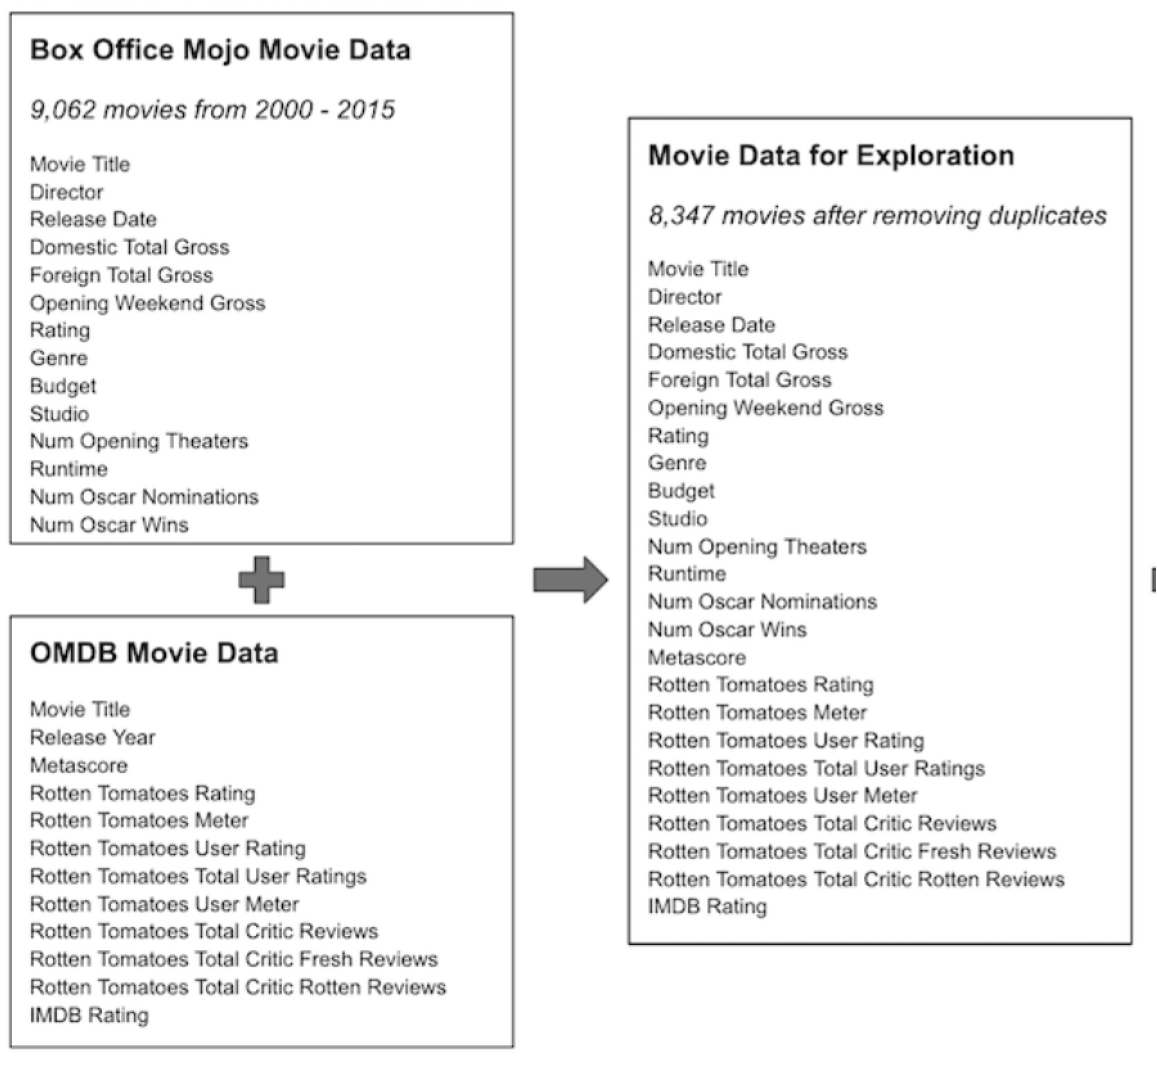
\includegraphics[scale=.75]{fds_image}

\pagebreak
\section*{Model}

A Decision Tree and Random Forest will be used to model film nomination for the Academy Awards. The features begin used to predict will be 
\begin{enumerate}
	\item critic review score
	\item audience review score
	\item directors previous nominations 
	\item directors previous awards (number of awards)
	\item Films previous awards (Globes, Bafta)
	\item Genre
	\item MPAA Rating
	\item Season (Spring, Summer, Holiday, Winter)
\end{enumerate} 

The correlation of the feature listed above with the target variable will be determined in the preliminary statistics. Both the Decision Tree and Random Forest will be able to give feature importance. Parameters for both models will need to optimized based on an average AUC on the ROC curve. The models will be evaluated using an ROC curve, AUC scores and cross validation. 

\section*{Assumptions and Limitations} 
Some assumption made at the begining of the project were that genre, season, other award, director reputation would have strong correlation with the target variable. Based on the model these features were not the most important features when determining whether a film receives an Oscar nomination. The assumption might be true if the data was more complete. 

When determining the reputation of the director it was found that only 227 different directors had been nominated for the Academy Awards and less than 88 directors had won. Given the large number of directors, the small portion of nominated directors did not make a significant impact to the target variable as assumed. This could be overcome by including director nominations from other major awards. 


Cleaning and merging the data sets proved difficult. Specifically finding common directors and films. For example Alejandro Gonzeles Innuritu had many different representation for his name. Also some films included extended title like The Avengers and Marvel's The Avengers. This made cleaning and merging the individual data sets difficult. Also removing duplicate entries based on film title could not be preformed because some films shared titles. This problem could be simplified if there was a consistent way to identify both director and film. 
  

Another limitation was many films do not report on their budget. This made it difficult to determine revenue. Therefore both features were dropped in the main analysis. Also it is unclear if budget includes marketing for the film. 

\section*{Problem in Scope of Class}

The goal of this project is to classify whether a film will be nominated for the Academy Awards. This is a classification problem utilizing the features listed above to determine the outcome of a film. As stated in the notebook, this model can be used to chose which films a studio campaigns for. 


\section*{Changes from Original Proposal}

There were a few features that were dropped from the initial proposal. Revenue was dropped because it could not be determined due to the large number of missing values for film budget. Also actors reputation was not considered because of the difficulty we had when merging names. Some other features that were dropped were the social impact of a film, buzzword analysis and script rating. 

\section*{Team Evaluation}

Alexander Rabinowitz: 5 \\
Khushnaseeb Ali: 5

\end{document}          
